\chapter{Jacobians} \label{ch:jacobians}
Problems in computer vision often involve nonlinear functions, such as camera projections and 3D transformations.
It is also common that these functions operate on and produce variables that are defined on manifolds, such as rotations on $\SO(3)$ and poses on $\SE(3)$.
As we will see in the following chapters, propagating uncertainty and estimating states from observations will typically involve linearising such functions with Taylor expansions.
Multivariate differentiation on vector spaces and Lie groups is therefore a key mathematical tool in vision-based state estimation.

This chapter will introduce useful notation and a procedure for computing derivatives on vector spaces and Lie groups based on \cite{SolaARobotics}.
We will finish this section with listing useful Jacobians for common operations on \SO(3) and \SE(3).

\section{Derivatives in vector spaces}
Let $f: \bbR^m \to \bbR^n$ be a multivariate function that takes vectors $\vecx \in \bbR^m$ as input and produces vectors $f(\vecx) \in \bbR^n$ as output.
The Jacobian matrix of $f$ is defined as the $n \times m$ matrix that stacks all the partial derivatives
%
\begin{equation} \label{eq:jacobian_def}
  \matJ = \dpar{f(\vecx)}{\vecx} \triangleq
  \begin{bmatrix}
    \dpar{f_1}{x_1} & \hdots & \dpar{f_1}{x_m}\\
    \vdots & & \vdots\\
    \dpar{f_n}{x_1} & \hdots & \dpar{f_n}{x_m}
  \end{bmatrix}
  \in \bbR^{n \times m}.
\end{equation}
%
Each column vector $\vecj_i = [\dpar{f_1}{x_i} \hdots \dpar{f_n}{x_i}]\trans$ of the Jacobian \eqref{eq:jacobian_def} corresponds to
%
\begin{equation} \label{eq:jacobian_column}
  \vecj_i = \dpar{f(\vecx)}{x_i} \triangleq \lim_{h \to 0} \frac{f(\vecx + h \vece_i) - f(\vecx)}{h} \in \bbR^n,
\end{equation}
%
where $\vece_i$ is the $i$-th natural basis vector of $\bbR^m$.
This represents the instantaneous variation of $f(\vecx)$ when $\vecx$ is perturbed in the direction of $\vece_i$.
We will in the following adopt the convenient notation from \cite{SolaARobotics}, where the Jacobian is given on the compact form
%
\begin{equation}  \label{eq:jacobian_sola_def}
  \matJ = \dpar{f(\vecx)}{\vecx} \triangleq
  \lim_{\vech \to 0} \frac{f(\vecx + \vech) - f(\vecx)}{\vech} \in \bbR^{n \times m},
\end{equation}
%
with $\vech \in \bbR^m$, which combines all the columns~\eqref{eq:jacobian_column} to form the definition of~\eqref{eq:jacobian_def}.
Like the Jacobian matrix in~\eqref{eq:jacobian_def}, the form used in~\eqref{eq:jacobian_sola_def} is just a notational convenience, since division by the vector $\vech$ is undefined, and proper computation requires~\eqref{eq:jacobian_column}.
However, by using this notation we can follow a straight-forward procedure to calculate Jacobians, by developing the numerator into a form linear in $\vech$ and identifying the left hand side as the Jacobian:
%
\begin{equation}  \label{eq:computing_jacobian}
  \lim_{\vech \to 0} \frac{f(\vecx + \vech) - f(\vecx)}{\vech} = \hdots =
  \lim_{\vech \to 0} \frac{\matJ \vech}{\vech} \triangleq \dpar{(\matJ \vech)}{\vech} = \matJ.
\end{equation}
%
To distinguish and identify different Jacobians, we will use the notation $\jac{f(\vecx)}{\vecx} \triangleq \dpar{f(\vecx)}{\vecx}$ and $\jac{\vecy}{\vecx} \triangleq \dpar{\vecy}{\vecx}$.

\begin{example}[frametitle=Computing the Jacobian $\jac{\matA \vecx}{\vecx}$]
For a vector $\vecx \in \bbR^m$ and a constant conformable matrix $\matA$, we want to compute the derivative of $f(\vecx) = \matA \vecx$ with respect to $\vecx$.
Using \eqref{eq:jacobian_sola_def} we get
\begin{subequations}
\begin{align}
  \jac{\matA \vecx}{\vecx} = \dpar{\matA \vecx}{\vecx} 
  &= \lim_{\vech \to 0} \frac{\matA (\vecx + \vech) - \matA \vecx}{\vech}\\[0.3em]
  &= \lim_{\vech \to 0} \frac{\matA \vecx + \matA \vech - \matA \vecx}{\vech}\\[0.3em]
  &= \lim_{\vech \to 0} \frac{\matA \vech}{\vech}\\[0.3em]
  &= \matA.
\end{align}
\end{subequations}
\end{example}

\begin{example}[frametitle=Computing the Jacobian $\jac{\vecx\trans \matA \vecx}{\vecx}$]
For a vector $\vecx \in \bbR^m$ and a constant matrix $\matA \in \bbR^{m \times m}$, we now want to compute the derivative of the scalar-valued quadratic form $f(\vecx) = \vecx\trans \matA \vecx$ with respect to $\vecx$.
By applying \eqref{eq:jacobian_sola_def} we get
\begin{subequations} \label{eq:jacobian_quadratic_form}
\begin{align}
  \jac{\vecx\trans \matA \vecx}{\vecx}
  &= \lim_{\vech \to 0} \frac{(\vecx + \vech)\trans \matA (\vecx + \vech) - \vecx\trans \matA \vecx}{\vech}\\
  &= \lim_{\vech \to 0} \frac{\vecx\trans \matA \vecx + \vech\trans \matA \vecx + \vecx\trans \matA \vech + \vech\trans \matA \vech - \vecx\trans \matA \vecx}{\vech}.\\
\intertext{By dropping the higher order term and using that for scalars $a\trans = a$, we get}
  \jac{\vecx\trans \matA \vecx}{\vecx}
  &= \lim_{\vech \to 0} \frac{\vecx\trans \matA \vech + (\vech\trans \matA \vecx)\trans}{\vech}\\[0.3em]
  &= \lim_{\vech \to 0} \frac{\vecx\trans \matA \vech + \vecx\trans \matA\trans \vech}{\vech}\\[0.3em]
  &= \lim_{\vech \to 0} \frac{\vecx\trans (\matA + \matA\trans) \vech}{\vech}\\[0.3em]
  &= \vecx\trans (\matA + \matA\trans).
\end{align}
\end{subequations}
\end{example}

For $\vecy = f(\vecx)$ and $\vecz = g(\vecy)$ we have $\vecz = g(f(\vecx))$.
The chain rule also applies in multivariate calculus, and lets us compute the derivative of $\vecz$ with respect to $\vecx$ as
\begin{equation}
  \dpar{\vecz}{\vecx} = \dpar{\vecz}{\vecy} \dpar{\vecy}{\vecx}.
\end{equation}
We can therefore express the Jacobian $\jac{\vecz}{\vecx}$ as a composition of several Jacobian blocks
\begin{equation}
  \jac{\vecz}{\vecx} = \jac{\vecz}{\vecy} \jac{\vecy}{\vecx}.
\end{equation}

\begin{example}[frametitle=Computing the Jacobian $\jac{\norm{\vecx - \veca}}{\vecx}$] \label{ex:jacobian-of-norm}
For a vector $\vecx \in \bbR^m$ and the constant vector $\veca \in \bbR^m$, we want to compute the derivative of the scalar-valued L2 norm of the difference between these vectors $f(\vecx) = \norm{\vecx - \veca}$ with respect to $\vecx$.
Using the chain rule, we can represent the Jacobian as
\begin{equation} \label{eq:jacobian_normdiff_blocks}
  \jac{\norm{\vecx - \veca}}{\vecx} = \jac{\norm{\vecx - \veca}}{\vecx - \veca} \jac{\vecx - \veca}{\vecx}.
\end{equation}
We can compute the first Jacobian by using the chain rule again:
\begin{equation}
  \jac{\norm{\vecx}}{\vecx} = \jac{\sqrt{\vecx\trans \vecx}}{\vecx\trans \vecx} \jac{\vecx\trans \vecx}{\vecx}.
\end{equation}
We can here recognise that $\jac{\sqrt{\vecx\trans \vecx}}{\vecx\trans \vecx}$ is simply $\dif{\sqrt{u}}{u}$ with $u = \vecx\trans \vecx$, and $\jac{\vecx\trans \vecx}{\vecx}$ is a special case of $\jac{\vecx\trans \matA \vecx}{\vecx}$ from \eqref{eq:jacobian_quadratic_form} with $\matA = \matI$.
This gives us
\begin{subequations} \label{eq:jacobian_norm}
\begin{align}
  \jac{\norm{\vecx}}{\vecx} 
  &= \jac{\sqrt{\vecx\trans \vecx}}{\vecx\trans \vecx} \jac{\vecx\trans \vecx}{\vecx}\\[0.3em]
  &= \frac{1}{2 \sqrt{\vecx\trans \vecx}} \; \vecx\trans(\matI + \matI\trans)\\[0.3em]
  &= \frac{2 \vecx\trans}{2 \norm{\vecx}}\\[0.3em]
  &= \frac{\vecx\trans}{\norm{\vecx}}.
\end{align}
\end{subequations}
By applying \eqref{eq:jacobian_sola_def} on the second Jacobian in \eqref{eq:jacobian_normdiff_blocks}, we see that
\begin{equation} \label{eq:jacobian_diff}
  \jac{\vecx - \veca}{\vecx} = \matI.
\end{equation}
We can now finally compose the Jacobian blocks \eqref{eq:jacobian_norm} and \eqref{eq:jacobian_diff} in \eqref{eq:jacobian_normdiff_blocks} to compute the desired Jacobian 
\begin{subequations} \label{eq:jacobian_normdiff}
\begin{align}
  \jac{\norm{\vecx - \veca}}{\vecx} 
  &= \jac{\norm{\vecx - \veca}}{\vecx - \veca} \jac{\vecx - \veca}{\vecx}\\[0.3em]
  &= \frac{(\vecx - \veca)\trans}{\norm{\vecx - \veca}} \; \matI\\[0.3em]
  &= \frac{(\vecx - \veca)\trans}{\norm{\vecx - \veca}}.
\end{align}
\end{subequations}
\end{example}

For small values of $\vech$, we have the linear first-order Taylor approximation
\begin{equation} \label{eq:linear-approximation}
  f(\vecx + \vech) \xrightarrow[\vech \to 0]{} f(\vecx) + \jac{f(\vecx)}{\vecx} \vech.
\end{equation}

This concludes our brief introduction to derivatives in vector spaces.
Those seeking further details should consult an appropriate text on multivariate calculus.
We will finish this section by emphasising that the procedure in \eqref{eq:jacobian_sola_def} is not applicable for 3D rotations and poses, which are defined on manifolds rather than on vector spaces.
The next section will describe how we apply the Lie theory from Chapter~\ref{sec:Lie-theory} to differentiate functions on these manifolds.

\section{Derivatives on Lie groups} \label{sec:derivative-Lie}
\begin{figure}[htb]
    \centering
    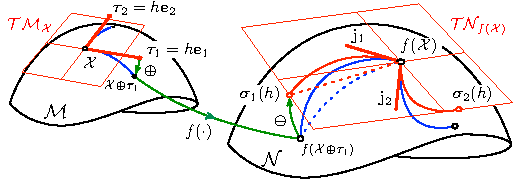
\includegraphics[width=0.9\columnwidth]{figures/jacobian.pdf}
    \caption{The right derivative of a function $f: \cM \to \cN$.
    The perturbation vectors in the canonical directions, $\vectau_i = h \vece_i \in \cT\cM_\cX$ are propagated to perturbation vectors $\vecsigma_i \in \cT\cN_{f(\cX)}$ through $\vecsigma_i(h) = f(\cX \oplus h \vece_i) \ominus f(\cX)$.
    The column vectors $\vecj_i$ of $\matJ$ are the derivatives $\vecj_i = \lim_{h \to 0} \vecsigma_i(h)/h$, and the Jacobian matrix $\matJ = [\vecj_1 \cdots \vecj_m]$ linearly maps tangent space vectors from $\cT\cM_\cX$ to $\cT\cN_{f(\cX)}$.\\
    (Image source: \cite{SolaARobotics}; licensed under \href{https://creativecommons.org/licenses/by-nc-sa/4.0/}{CC BY-NC-SA 4.0})}
    \label{fig:lie-jacobian}
\end{figure}

For functions acting on Lie groups, we can express the derivative similarly to that of \eqref{eq:jacobian_sola_def} by using the $\oplus$ and $\ominus$ operators from Section~\ref{sec:lie-plus-and-minus} with infinitesimal perturbations in the tangent space.
For a function $f : \cM \to \cN$, the right (local) derivative is given by
\begin{align}
  \jac{}{} = \frac{^{\cX} \partial f(\cX)}{\partial \cX} &\triangleq 
  \lim_{\vectau \to 0} \frac{f(\cX \oplus \vectau) \ominus f(\cX)}{\vectau} \in \bbR^{n \times m} \label{eq:lie-derivative}\\
  &= \lim_{\vectau \to 0} \frac{\Log \left( f(\cX)^{-1} \circ f(\cX \circ \Exp(\vectau)) \right)}{\vectau},
\end{align}
where $\vectau \in \cT\cM_\cX$.

Variations in $\cX$ and $f(\cX)$ are here expressed in terms of vectors in the local tangent spaces at $\cX \in \cM$ and $f(\cX) \in \cN$ respectively.
The tangent space vector
\begin{equation}
  \vecsigma_i(h) = f(\cX \oplus h \vece_i) \ominus f(\cX) \quad \in \cT\cN_{f(\cX)}
\end{equation}
is the variation of $f(\cX)$ when $\cX$ is perturbed in the direction of $\vece_i$.
The column vectors $\vecj_i$ of the Jacobian are the derivatives $\vecj_i = \lim_{h \to 0} \vecsigma_i(h)/h$, and $\matJ = [\vecj_1 \cdots \vecj_m]$ is a proper Jacobian matrix in $\bbR^{n \times m}$, linearly mapping the local tangent spaces $\cT\cM_\cX \to \cT\cN_{f(\cX)}$ (Figure~\ref{fig:lie-jacobian}).

As in the previous section, we can use \eqref{eq:lie-derivative} to compute the Jacobians by applying the same procedure as in \eqref{eq:computing_jacobian}.

\begin{example}[frametitle=Computing the Jacobian $\jac{\cX \circ \cY}{\cY}$ on the manifold]
We can compute the Jacobian of the composition $\cX \circ \cY$ between two elements $\cX, \cY \in \cM$ with respect to $\cY$, by using \eqref{eq:lie-derivative} with the procedure in \eqref{eq:computing_jacobian}.

\begin{subequations}
\begin{align}
  \jac{\cX \circ \cY}{\cY} &= \lim_{\vectau \to 0} 
  \frac{(\cX \circ (\cY \oplus \vectau)) \ominus (\cX \circ \cY)}{\vectau}\\
  &= \lim_{\vectau \to 0} 
  \frac{\Log \left( (\cX \circ \cY)^{-1} \circ (\cX \circ (\cY \circ \Exp(\vectau))) \right)}{\vectau}\\
  &= \lim_{\vectau \to 0} 
  \frac{\Log \left( (\cX \circ \cY)^{-1} (\cX \circ \cY) \circ \Exp(\vectau) \right)}{\vectau}\\
  &= \lim_{\vectau \to 0} 
  \frac{\vectau}{\vectau}\\
  &= \matI.
\end{align}
\end{subequations}
\end{example}

For small values of $\vectau$, the following first-order Taylor approximation holds,
\begin{equation} \label{eq:lie-linearisation}
  f(\cX \oplus \vectau) \xrightarrow[\vectau \to 0]{}
  f(\cX) \oplus \jac{f(\cX)}{\cX} \vectau,
\end{equation}
and can be used to linearise the function $f(\cX)$ on the manifold, similarly to \eqref{eq:linear-approximation}.

We can apply left perturbations to compute the corresponding left (global) derivative \cite{SolaARobotics}.
The left derivative is also related to the right (local) derivative by the adjoints of $\cM$ and $\cN$
\begin{equation}
  \frac{^{\cE} \partial f(\cX)}{\partial \cX} \mAd_\cX = \mAd_{f(\cX)} \frac{^{\cX} \partial f(\cX)}{\partial \cX}
\end{equation}
so that
\begin{equation}
  \frac{^{\cE} \partial f(\cX)}{\partial \cX} = \mAd_{f(\cX)} \frac{^{\cX} \partial f(\cX)}{\partial \cX} {\mAd_\cX}^{-1}.
\end{equation}

It can be shown that the chain rule also applies to derivatives on the manifold (as long as we do not mix right and left derivatives) \cite{SolaARobotics}.
This means that for $\cY = f(\cX)$ and $\cZ = g(\cY)$, we have $\cZ = g(f(\cX))$ and
\begin{equation}
  \dpar{\cZ}{\cX} = \dpar{\cZ}{\cY} \dpar{\cY}{\cX} \quad\quad \text{or} \quad\quad \jac{\cZ}{\cX} = \jac{\cZ}{\cY} \jac{\cY}{\cX}.
\end{equation}

\section{Elementary Lie group Jacobian blocks} \label{sec:elem-lie-blocks}
With the derivative properly defined, we are able to compute the Jacobians for the common operations on Lie groups that are listed here.
We will use these elementary Jacobians to define the corresponding Jacobians for $\SO(3)$ and $\SE(3)$ in Section~\ref{sec:Jacobians-SO3} and Section~\ref{sec:Jacobians-SE3}.
With the chain rule, these Jacobians are the elementary building blocks for expressing the derivative of functions operating on orientations and poses. 

\subsection{Jacobian of the inverse operation}
The Jacobian of the inverse operation is given by
\begin{equation} \label{eq:inverse-lie-jacobian}
  \jac{\cX^{-1}}{\cX} = -\mAd_\cX.
\end{equation}

\subsection{Jacobians of the composition operation}
For $\cX, \cY \in \cM$, the Jacobians of the composition operation is given by
\begin{align}
  \jac{\cX \circ \cY}{\cX} &= {\mAd_\cY}^{-1}\\
  \jac{\cX \circ \cY}{\cY} &= \matI.
\end{align}

\subsection{Jacobians of the group action}
For $\cX \in \cM$ and $v \in \cV$, the Jacobians of the group action $\cX \cdot v$ is defined as
\begin{align}
  \jac{\cX \cdot v}{\cX} \triangleq \frac{\prescript{\cX}{}{\partial}(\cX \cdot v)}{\partial \cX}\\
  \jac{\cX \cdot v}{v} \triangleq \frac{\prescript{v}{}{\partial}(\cX \cdot v)}{\partial v}.
\end{align}
Since the group action depends on $\cV$, these expressions cannot be generalised.
The following examples show how to compute these Jacobians for $\SO(3)$ and $\SE(3)$.

\begin{example}[frametitle=Computing the Jacobians for $\matR \cdot \vecx$] \label{ex:lie-group-action-jac-SO3-example}
For a rotation matrix $\matR \in \SO(3)$ and a vector $\vecx \in \bbR^3$, the group action of $\matR$ on $\vecx$ is defined in \eqref{eq:SO3-group-action} as $\matR \cdot \vecx \triangleq \matR \vecx$.

The Jacobian of $\matR \cdot \vecx$ with respect to $\matR$ is given by
\begin{subequations}
\begin{align}
  \jac{\matR \cdot \vecx}{\matR} &= \lim_{\vectheta \to 0} 
  \frac{(\matR \oplus \vectheta) \cdot \vecx - (\matR \cdot \vecx)}{\vectheta}\\
  &= \lim_{\vectheta \to 0} 
  \frac{(\matR \circ \Exp(\vectheta)) \cdot \vecx - (\matR \cdot \vecx)}{\vectheta}.\\
  \intertext{Since we are interested in the limit where $\vectheta \to 0$, we can use the approximation $\Exp(\vectheta) \approx \matI + \vectheta^\wedge$ from \eqref{eq:SO3-Exp-approx}. By also switching to matrix operations, we get}
  &= \lim_{\vectheta \to 0} 
  \frac{\matR (\matI + [\vectheta]_\times) \vecx - \matR \vecx}{\vectheta}\\
  &= \lim_{\vectheta \to 0} 
  \frac{\matR \vecx + \matR [\vectheta]_\times \vecx - \matR \vecx}{\vectheta}\\
  &= \lim_{\vectheta \to 0} 
  \frac{\matR [\vectheta]_\times \vecx}{\vectheta}.\\
  \intertext{With the property $\skewsymm{\veca}\vecb = -\skewsymm{\vecb}\veca$, we get the desired form}
  &= \lim_{\vectheta \to 0} 
  \frac{-\matR [\vecx]_\times \vectheta}{\vectheta},\\
  \intertext{which results in the Jacobian}
  &= -\matR [\vecx]_\times.
\end{align}
\end{subequations}

The Jacobian of $\matR \cdot \vecx$ with respect to $\vecx$ is given by
\begin{subequations}
\begin{align}
  \jac{\matR \cdot \vecx}{\vecx} &= \lim_{\partial \vecx \to 0} 
  \frac{\matR \cdot (\vecx + \partial \vecx) - (\matR \cdot \vecx)}{\partial \vecx}\\
  &= \lim_{\partial \vecx \to 0} 
  \frac{\matR \vecx + \matR \partial \vecx - \matR \vecx}{\partial \vecx}\\
  &= \lim_{\partial \vecx \to 0} 
  \frac{\matR \partial \vecx}{\partial \vecx}\\
  &= \matR.
\end{align}
\end{subequations}
\end{example}

\begin{example}[frametitle=Computing the Jacobians for $\matT \cdot \vecx$] \label{ex:lie-group-action-jac-SE3-example}
For a pose $\matT = \begin{bsmallmatrix} \matR & \vect\\ \matr{0}\trans & 1 \end{bsmallmatrix} \in \SE(3)$ and a vector $\vecx \in \bbR^3$, the group action of $\matT$ on $\vecx$ is defined in \eqref{eq:SE3-group-action} as $\matT \cdot \vecx \triangleq \matR \vecx + \vect$.

The Jacobian of $\matT \cdot \vecx$ with respect to $\matT$ is given by
\begin{subequations}
\begin{align}
  \jac{\matT \cdot \vecx}{\matT} &= \lim_{\vecxi \to 0} 
  \frac{(\matT \oplus \vecxi) \cdot \vecx - (\matT \cdot \vecx)}{\vecxi}\\
  &= \lim_{\vecxi \to 0} 
  \frac{(\matT \circ \Exp(\vecxi)) \cdot \vecx - (\matT \cdot \vecx)}{\vecxi}.\\
  \intertext{Since we are interested in the limit where $\vecxi \to 0$, we can use the approximation $\Exp(\vecxi) \approx \matI + \vecxi^\wedge$ from \eqref{eq:SE3-Exp-approx}.}
  &= \lim_{\vecxi \to 0} 
  \frac{\matT \circ (\matI + \vecxi^\wedge) \cdot \vecx - (\matT \cdot \vecx)}{\vecxi}\\
  &= \lim_{\vecxi \to 0} 
  \frac{ \matT \circ
  \begin{bmatrix}
    \matI + \skewsymm{\vectheta} & \vecrho\\
    \matr{0}\trans & 1
  \end{bmatrix} \cdot \vecx - (\matT \cdot \vecx)}{\vecxi}.\\
  \intertext{By performing the composition as matrix multiplication,}
  &= \lim_{\vecxi \to 0} 
  \frac{
  \begin{bmatrix}
    \matR(\matI + \skewsymm{\vectheta}) & \matR\vecrho + \vect\\
    \matr{0}\trans & 1
  \end{bmatrix} \cdot \vecx - (\matT \cdot \vecx)}{\vecxi},\\
  \intertext{and performing the group action according to \eqref{eq:SE3-group-action},}
  &= \lim_{\vecxi \to 0} 
  \frac{\matR(\matI + [\vectheta]_\times)\vecx + \matR\vecrho + \vect - (\matR\vecx + \vect)}{\vecxi},\\
  \intertext{we get}
  &= \lim_{\vecxi \to 0} 
  \frac{\matR\vecx + \matR\skewsymm{\vectheta}\vecx + \matR\vecrho + \vect - \matR\vecx - \vect}{\vecxi}\\
  &= \lim_{\vecxi \to 0} 
  \frac{\matR\vecrho + \matR\skewsymm{\vectheta}\vecx}{\vecxi}.\\
  \intertext{With the property $\skewsymm{\veca}\vecb = -\skewsymm{\vecb}\veca$, we get the desired form}
  &= \lim_{\vecxi \to 0} 
  \frac{\matR\vecrho - \matR\skewsymm{\vecx}\vectheta}{\vecxi}\\
  &= \lim_{\vecxi \to 0} 
  \frac{
  \begin{bmatrix}
    \matR & -\matR[\vecx]_\times
  \end{bmatrix}
  \vecxi}{\vecxi},\\
  \intertext{which results in the Jacobian}
  &= 
  \begin{bmatrix}
    \matR & -\matR[\vecx]_\times
  \end{bmatrix}.
\end{align}
\end{subequations}

The Jacobian of $\matT \cdot \vecx$ with respect to $\vecx$ is given by
\begin{subequations}
\begin{align}
  \jac{\matT \cdot \vecx}{\vecx} &= \lim_{\partial \vecx \to 0} 
  \frac{\matT \cdot (\vecx + \partial \vecx) - (\matT \cdot \vecx)}{\partial \vecx}\\
  &= \lim_{\partial \vecx \to 0} 
  \frac{\matR(\vecx + \partial \vecx) + \vect - (\matR\vecx + \vect)}{\partial \vecx}\\
  &= \lim_{\partial \vecx \to 0} 
  \frac{\matR\vecx + \matR\partial\vecx + \vect - \matR\vecx -\vect}{\partial \vecx}\\
  &= \lim_{\partial \vecx \to 0} 
  \frac{\matR\partial\vecx}{\partial \vecx}\\
  &= \matR.
\end{align}
\end{subequations}
\end{example}

\subsection{Jacobians of $\cM$}
The right Jacobian of $\cM$ is defined as the right derivative of $\cX = \Exp(\vectau)$
\begin{equation} \label{eq:right-jacobian}
  \jac{}{r}(\vectau) \triangleq \frac{\prescript{\cX}{}{\partial}\Exp(\vectau)}{\partial \vectau} \in \bbR^{m \times m},
\end{equation}
where $\vectau \in \bbR^m$.

The right Jacobian maps variations of the vector $\vectau$ into variations in the \emph{local} tangent space at $\cX = \Exp(\vectau)$.
For small $\delta \vectau$, the following approximations hold
\begin{align}
  \Exp(\vectau + \delta \vectau) &\approx \Exp(\vectau) \Exp(\jac{}{r}(\vectau) \delta \vectau)\\
  \Exp(\vectau) \Exp(\delta \vectau) &\approx \Exp(\vectau + \jac{}{r}^{-1}(\vectau) \delta \vectau)\\
  \Log(\Exp(\vectau) \Exp(\delta \vectau)) &\approx \vectau + \jac{}{r}^{-1}(\vectau)\delta\vectau. \label{eq:Log-approx}
\end{align}

For $\vectau = \Log(\cX)$, we have from \eqref{eq:Log-approx} that the Jacobian of the $\Log$ operation is given by
\begin{equation}
  \jac{\Log(\cX)}{\cX} \triangleq \frac{\prescript{\cX}{}{\partial \Log(\cX)}}{\partial \cX} = \jac{}{r}^{-1}(\vectau).
\end{equation}

The corresponding left Jacobian
\begin{equation}
  \jac{}{l}(\vectau) \triangleq \frac{\prescript{\cE}{}{\partial}\Exp(\vectau)}{\partial \vectau} \in \bbR^{m \times m},
\end{equation}
maps variation of $\vectau$ into variations in the \emph{global} tangent space.
We can relate the left and right Jacobians with the adjoint matrix:
\begin{equation} \label{eq:right-adjoin-left-jacobians}
  \mAd_{\Exp(\vectau)} = \jac{}{l}(\vectau) \jac{}{r}^{-1}(\vectau).
\end{equation}
Also, as shown in Example~\ref{ex:chain-rule-left-jac} below, applying the chain rule to $\jac{}{r}(-\vectau)$ gives us
\begin{equation} \label{eq:lie-right-jac-from-left}
  \jac{}{r}(-\vectau) = \jac{}{l}(\vectau).
\end{equation}

\begin{example}[frametitle=Applying the chain rule to $\jac{}{r}(-\vectau)$] \label{ex:chain-rule-left-jac}
The definition of the right Jacobian \eqref{eq:right-jacobian} gives us
\begin{subequations}
\begin{align}
  \jac{}{r}(-\vectau) &= \jac{\Exp(-\vectau)}{-\vectau}.\\ 
  \intertext{Since $\Exp(-\vectau) = \Exp(\vectau)^{-1}$, we can express this as}
  &= \jac{\Exp(\vectau)^{-1}}{-\vectau}.\\
  \intertext{By applying the chain rule and using \eqref{eq:right-adjoin-left-jacobians} and \eqref{eq:inverse-lie-jacobian}, we get}
  &= \jac{\Exp(\vectau)^{-1}}{\Exp(\vectau)} \jac{\Exp(\vectau)}{\vectau} \jac{\vectau}{-\vectau}\\
  &= -\mAd_{\Exp(\vectau)} \jac{}{r}(\vectau) (-\matI)\\
  &= \jac{}{l}(\vectau).
\end{align}
\end{subequations}
\end{example}

\subsection{Jacobians of the plus and minus operators}
The Jacobians of the plus and minus operators can be derived by applying the chain rule to the definitions in \eqref{eq:lie-plus-def} and \eqref{eq:lie-minus-def}.
We have
\begin{align}
  \jac{\cX \oplus \vectau}{\cX} &= {\mAd_{\Exp(\vectau)}}^{-1}\\
  \jac{\cX \oplus \vectau}{\vectau} &= \jac{}{r}(\vectau),
\end{align}
and with $\vectau = \cY \ominus \cX$,
\begin{align}
  \jac{\cY \ominus \cX}{\cX} &= -\jac{}{l}^{-1}(\vectau)\\
  \jac{\cY \ominus \cX}{\cY} &= \jac{}{r}^{-1}(\vectau).
\end{align}

\section{Jacobian blocks for \SO(3)} \label{sec:Jacobians-SO3}
The right and left Jacobians, and their inverses, have the following closed form expressions: 
\begin{align}
\jac{}{r}(\vectheta) &= \matI - \frac{1-\cos\theta}{\theta^2}\skewsymm{\vectheta} + \frac{\theta-\sin\theta}{\theta^3}\skewsymm{\vectheta}^2\\
\jac{}{r}^{-1}(\vectheta) &= \matI + \frac{1}{2}\skewsymm{\vectheta} + \left(\frac{1}{\theta^2} - \frac{1+\cos\theta}{2\theta\sin\theta}\right)\skewsymm{\vectheta}^2 \\
\jac{}{l}(\vectheta) &= \matI + \frac{1-\cos\theta}{\theta^2}\skewsymm{\vectheta} + \frac{\theta-\sin\theta}{\theta^3}\skewsymm{\vectheta}^2 \label{eq:SO3-left-jac}\\
\jac{}{l}^{-1}(\vectheta) &= \matI - \frac{1}{2}\skewsymm{\vectheta} + \left(\frac{1}{\theta^2} - \frac{1+\cos\theta}{2\theta\sin\theta}\right)\skewsymm{\vectheta}^2.
\end{align}
Notice that
\begin{equation}
  \jac{}{l}(\vectheta) = \jac{}{r}(\vectheta)\trans, \quad\quad \jac{}{l}(\vectheta)^{-1} = \jac{}{r}(\vectheta)\invtrans.
\end{equation}

In the remainder of this section, we list the Jacobian blocks in Section~\ref{sec:elem-lie-blocks} developed for $\SO(3)$.

\subsection{Jacobian of the inverse operation}
\begin{equation}
  \jac{\matR^{-1}}{\matR} = -\mAd_\matR = -\matR.
\end{equation}

\subsection{Jacobians of the composition operation}
\begin{align}
  \jac{\matR_a \matR_b}{\matR_a} &= {\mAd_{\matR_b}}^{-1} = \matR_b\trans\\
  \jac{\matR_a \matR_b}{\matR_b} &= \matI.
\end{align}

\subsection{Jacobians of the group action}
From Example~\ref{ex:lie-group-action-jac-SO3-example} we have
\begin{align}
  \jac{\matR \cdot \vecx}{\matR} &= -\matR [\vecx]_\times\\
  \jac{\matR \cdot \vecx}{\vecx} &= \matR.
\end{align}

\subsection{Jacobians of the plus and minus operators}
\begin{align}
  \jac{\matR \oplus \vectheta}{\matR} &= {\mAd_{\Exp(\vectheta)}}^{-1} = \matR(\vectheta)\trans\\
  \jac{\matR \oplus \vectheta}{\vectheta} &= \jac{}{r}(\vectheta).
\end{align}
For $\vectheta = \matR_b \ominus \matR_a$, we have
\begin{align}
  \jac{\matR_b \ominus \matR_a}{\matR_a} &= -\jac{}{l}^{-1}(\vectheta)\\
  \jac{\matR_b \ominus \matR_a}{\matR_b} &= \jac{}{r}^{-1}(\vectheta).
\end{align}

\section{Jacobian blocks for \SE(3)} \label{sec:Jacobians-SE3}
The left Jacobian and its inverse have the following closed form expressions: 
\begin{align}
\jac{}{l}(\vecxi) &= 
\begin{bmatrix}
  \jac{}{l}(\vectheta) & \matQ(\vecxi) \\
  \matr{0} & \jac{}{l}(\vectheta)
\end{bmatrix}\\
\jac{}{l}^{-1}(\vecxi) &= 
\begin{bmatrix}
  \jac{}{l}^{-1}(\vectheta) & -\jac{}{l}^{-1}(\vectheta) \matQ(\vecxi) \jac{}{l}^{-1}(\vectheta) \\
  \matr{0} & \jac{}{l}^{-1}(\vectheta)
\end{bmatrix}.  \label{eq:jacobian-left-inverse-SE3}
\end{align}
Here $\jac{}{l}(\vectheta)$ is the left Jacobian of $\SO(3)$ in \eqref{eq:SO3-left-jac} and $\matQ(\vecxi)$ is given by
%
\newcommand{\rhox}{\skewsymm{\vecrho}}
\newcommand{\thetax}{\skewsymm{\vectheta}}
%
\begin{equation}
\begin{split}
\matQ(\vecxi) =& 
  \frac{1}{2}\rhox 
  + \frac{\theta - \sin\theta}{\theta^3}(\thetax\rhox+\rhox\thetax+\thetax\rhox\thetax)\\
  &- \frac{1 - \frac{\theta^2}{2} - \cos\theta}{\theta^4}(\thetax^2\rhox+\rhox\thetax^2-3\thetax\rhox\thetax)\\
  &-\frac{1}{2}\left(\frac{1 -  \frac{\theta^2}{2} - \cos\theta}{\theta^4} 
                  - 3\frac{\theta-\sin\theta-\frac{\theta^3}{6}}{\theta^5}\right)
                  (\thetax\rhox\thetax^2 + \thetax^2\rhox\thetax).
\end{split}
\end{equation}
%
The right Jacobian and its inverse can be obtained using \eqref{eq:lie-right-jac-from-left}.

In the remainder of this section, we list the Jacobian blocks in Section~\ref{sec:elem-lie-blocks} developed for $\SE(3)$.

\subsection{Jacobian of the inverse operation}
\begin{equation}
  \jac{\matT^{-1}}{\matT} = -\mAd_\matT = -
  \begin{bmatrix}
    \matR & \skewsymm{\vect}\matR\\
    \matr{0} & \matR
  \end{bmatrix}.
\end{equation}

\subsection{Jacobians of the composition operation}
\begin{align}
  \jac{\matT_a \matT_b}{\matT_a} &= {\mAd_{\matT_b}}^{-1} = 
  \begin{bmatrix}
    \matR_b\trans & -\matR_b\trans \skewsymm{\vect_b}\\
    \matr{0} & \matR_b\trans
  \end{bmatrix}\\
  \jac{\matT_a \matT_b}{\matT_b} &= \matI.
\end{align}

\subsection{Jacobians of the group action}
From Example~\ref{ex:lie-group-action-jac-SE3-example} we have
\begin{align}
  \jac{\matT \cdot \vecx}{\matT} &= 
  \begin{bmatrix}
    \matR & -\matR\skewsymm{\vecx}
  \end{bmatrix}\\
  \jac{\matT \cdot \vecx}{\vecx} &= \matR.
\end{align}

\subsection{Jacobians of the plus and minus operators}
\begin{align}
  \jac{\matT \oplus \vecxi}{\matT} &= {\mAd_{\Exp(\vecxi)}}^{-1}\\
  \jac{\matT \oplus \vecxi}{\vecxi} &= \jac{}{r}(\vecxi).
\end{align}
For $\vecxi = \matT_b \ominus \matT_a$, we have
\begin{align}
  \jac{\matT_b \ominus \matT_a}{\matT_a} &= -\jac{}{l}^{-1}(\vecxi)  \label{eq:jacobian-minus-x-SE3}\\
  \jac{\matT_b \ominus \matT_a}{\matT_b} &= \jac{}{r}^{-1}(\vecxi).
\end{align}
